% =====================================================================
% PARTIE 8 : LE DASHBOARD DE DEMONSTRATION (etude informatique v2.4, partie III)
\clearpage
\partieENO{Le dashboard de démonstration}

Cette partie reprend en entier l'étude de la copie de démonstration du dashboard. Le dashboard réel ne peut tourner qu'avec la tour branchée ; je veux pouvoir le montrer à n'importe qui, sur n'importe quel ordinateur, sans matériel.

Je commence par donner le lien vers le dashboard de démonstration en ligne (9.1), pour qu'on puisse l'ouvrir tout de suite. Je présente ensuite l'objectif et la démarche (9.2), puis je décris l'architecture (9.3). Je détaille le faux Arduino et les calculs qui le font fonctionner (9.4), puis l'accès et le premier lancement (9.5). Je présente enfin les tests et les résultats (9.6), et le dashboard publié en ligne avec ses captures (9.7).

% ---------------------------------------------------------------------
\subsection{Lien vers le dashboard de démonstration}

Le dashboard de démonstration est publié en ligne : il s'ouvre dans un navigateur, sans rien installer. Depuis le 20 novembre 2026, la page publiée est celle de la tour elle-même, avec la simulation embarquée : les mesures évoluent au fil du temps au lieu d'être figées.

\textbf{Lien :} \href{https://claude.ai/artifact/KExrrcoxh41KNf55szF4Wk}{\textbf{ouvrir le dashboard de démonstration}}

\textbf{Adresse complète :} \url{https://claude.ai/artifact/KExrrcoxh41KNf55szF4Wk}

\textbf{Connexion.} La page s'ouvre sur l'écran de connexion. L'identifiant est \texttt{demo} et le mot de passe est \texttt{hydrotour-demo}. Il faut aussi recopier les cinq caractères du code affiché ; le bouton « Autre image » en génère un nouveau. Les quatre onglets se parcourent ensuite comme sur la tour, écran d'étalonnage compris. Les ordres envoyés aux pompes agissent sur la simulation, jamais sur du matériel. Deux actions disent qu'elles ne sont pas disponibles en ligne, parce qu'elles demandent la tour : le téléchargement des fichiers CSV et les boutons d'étalonnage.

\textbf{Accès.} La page est privée : seules les personnes à qui je donne l'accès peuvent l'ouvrir. Les parties 9.2 à 9.7 expliquent comment cette copie est construite et ce qu'elle montre.

% ---------------------------------------------------------------------
\subsection{Objectif et démarche}

Cette sous-partie dit d'abord ce que je veux obtenir, puis les choix que je fais pour y arriver, et enfin l'ordre dans lequel je travaille.

\subsubsection*{Ce que je veux obtenir}

Je dispose d'un dashboard qui pilote la vraie tour hydroponique : il lit un Arduino, décide de l'état des pompes et affiche tout dans une page protégée par un identifiant, un mot de passe et un captcha. Ce dashboard ne peut tourner qu'avec le matériel branché. Je veux donc en faire une copie exacte qui fonctionne sans aucun matériel, avec son propre identifiant et son propre mot de passe, pour pouvoir la montrer à n'importe qui.

Le point difficile est le mot « exacte ». Si je me contente de refaire une page qui ressemble à l'original avec des chiffres figés, je ne montre rien du système réel. Je préfère garder le vrai serveur, le vrai pilote et la vraie page, et ne remplacer que ce qui ne peut pas exister sans matériel : la carte Arduino.

\subsubsection*{Les choix que je fais}

Je compare trois façons de faire. La première est une page statique avec des valeurs écrites en dur : c'est simple, mais les courbes ne bougent pas, les boutons ne font rien et la connexion n'existe pas. La deuxième est d'envoyer de fausses mesures au vrai serveur avec le script \texttt{fausses\_mesures.py} qui existe déjà : les courbes vivent, mais la tour reste sans réaction, car le pilote ne tourne que s'il y a un Arduino. La troisième est de remplacer l'Arduino par une classe qui a la même interface mais qui simule la tour : tout le reste du programme tourne comme sur la vraie tour.

Je retiens la troisième. Elle demande un seul nouveau fichier et trois petites modifications, et elle a un avantage fort : quand une pompe s'allume dans la démonstration, la simulation réagit, donc le pilote voit son effet et décide la suite, exactement comme sur la tour.

\begin{aretenir}
La démo n'est pas un décor : le serveur, le pilote, la page et l'accès sont ceux de la vraie tour. Seule la carte Arduino est simulée.
\end{aretenir}

\subsubsection*{L'ordre de travail}

Je commence par retrouver le code du dashboard dans le dossier \texttt{HYDROCODE/SERVEUR} et par lire comment le serveur parle à l'Arduino. Ensuite je copie les fichiers utiles dans un nouveau dossier \texttt{HYDROCODE/DEMO}, sans toucher à l'original. J'écris le faux Arduino, puis j'adapte l'accès et le premier lancement. Enfin je lance le serveur, je teste chaque route et je relève les données.

% ---------------------------------------------------------------------
\Needspace{8\baselineskip}\subsection{Architecture}

Cette sous-partie décrit d'abord comment les éléments du programme se parlent, ensuite quels fichiers je copie, modifie ou crée, puis le déroulement d'un tour de mesure.

\subsubsection*{Vue d'ensemble}

Je cherche à montrer ce qui change entre la tour réelle et la démonstration. Le serveur \texttt{server.py} lit une carte à travers un objet qui s'appelle \texttt{Arduino} et qui offre une dizaine de méthodes (lire le pH, lire la batterie, allumer une pompe, etc.). Si je fournis un autre objet avec les mêmes méthodes, le serveur ne voit pas la différence. C'est ce que fait \texttt{arduino\_demo.py}.

Le schéma suivant montre l'architecture de la démonstration.

\begin{figure}[H]
\centering
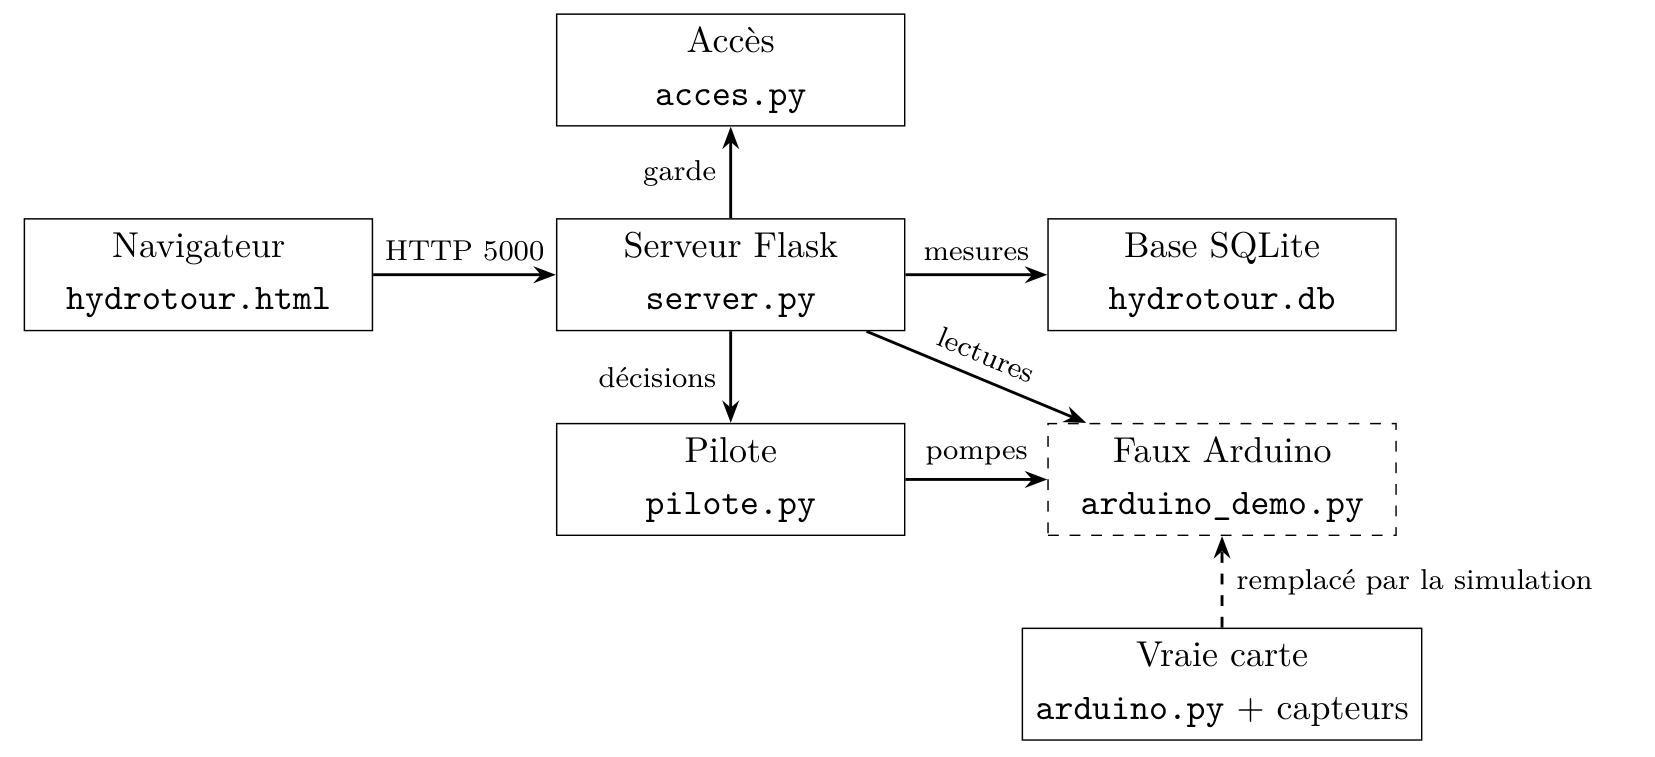
\includegraphics[width=0.85\textwidth]{img/inf/h_archi.png}
\caption{Architecture de la démo. Trait pointillé : l'élément qui remplace le matériel.}
\end{figure}

\subsubsection*{Les fichiers du dossier de démonstration}

Pour chaque fichier, je note s'il est copié tel quel, modifié ou nouveau. Je garde l'original intact dans \texttt{SERVEUR} : le dossier \texttt{DEMO} est une copie indépendante qu'on peut déplacer ou publier sans risque pour la vraie tour.

Le tableau suivant liste les fichiers de la démonstration.

\begin{table}[H]
\centering
\small
\begin{tabularx}{\textwidth}{|l|l|r|Y|}
\hline
\textbf{Fichier} & \textbf{État} & \textbf{Lignes} & \textbf{Rôle} \\
\hline
\texttt{hydrotour.html} & copié & 2097 & La page du dashboard \\
\hline
\texttt{pilote.py} & copié & 249 & Cycle de la pompe, batterie, dosage \\
\hline
\texttt{fausses\_mesures.py} & copié & 139 & Génère l'historique de départ \\
\hline
\texttt{server.py} & modifié & 544 & Serveur ; 22 lignes ajoutées \\
\hline
\texttt{acces.py} & modifié & 297 & Connexion ; 2 lignes ajoutées \\
\hline
\texttt{arduino\_demo.py} & nouveau & 134 & Simule la carte Arduino \\
\hline
\texttt{lancer\_demo.bat} & nouveau & 4 & Installe Flask et Pillow puis lance \\
\hline
\end{tabularx}
\caption{Fichiers de la démo.}
\end{table}

\subsubsection*{Un tour de mesure}

Le serveur répète le même tour toutes les \qty{10}{s}. Il lit les capteurs, convertit les valeurs brutes en grandeurs physiques, laisse le pilote décider, enregistre la ligne dans la base, puis attend. Comme la conversion se fait dans le serveur et non dans la carte, le faux Arduino doit renvoyer des valeurs brutes (millivolts, ohms) : c'est ce qui garantit que les conversions et l'étalonnage de la vraie tour sont aussi exercés.

L'organigramme suivant décrit la boucle de mesure du serveur.

\begin{figure}[H]
\centering
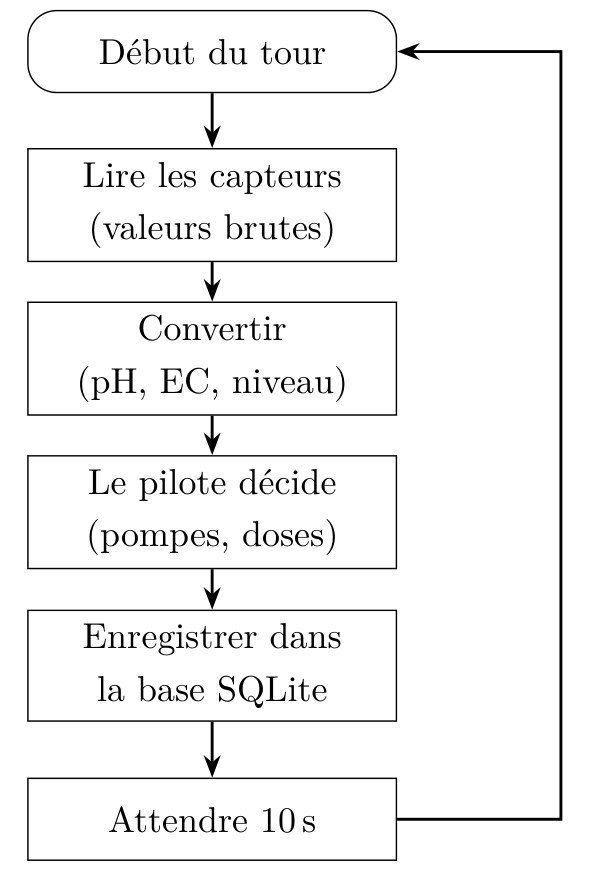
\includegraphics[width=0.42\textwidth]{img/inf/h_boucle.png}
\caption{Boucle de mesure du serveur (organigramme, ISO 5807).}
\end{figure}

% ---------------------------------------------------------------------
\Needspace{8\baselineskip}\subsection{Le faux Arduino}

Cette sous-partie explique d'abord le principe de la simulation. Elle présente ensuite les calculs qui transforment l'état simulé en valeurs brutes (pH, EC, niveau), puis le bilan d'énergie de la batterie, et enfin la façon dont les pompes agissent sur l'état.

\subsubsection*{Le principe}

Je cherche un modèle assez simple pour être écrit en cent lignes, mais assez réaliste pour que le pilote ait des décisions à prendre. L'état de la tour tient en quelques variables : le pH, l'EC, le niveau d'eau, la température de l'eau et la charge de la batterie. À chaque lecture, le temps réel écoulé depuis la dernière lecture fait avancer ces variables. Je plafonne ce temps à \qty{60}{s} pour qu'une mise en veille du PC ne fasse pas sauter la simulation.

Je choisis un temps réel et non un temps accéléré : le cycle de la pompe dure \qty{15}{min} en marche puis \qty{15}{min} à l'arrêt, et le soleil suit l'heure du PC. Une démonstration fidèle montre donc une vraie journée.

\begin{table}[H]
\centering
\small
\begin{tabularx}{\textwidth}{|l|l|Y|}
\hline
\textbf{Variable} & \textbf{Départ} & \textbf{Évolution sans intervention} \\
\hline
pH & 5,9 & monte de 0,002 par minute \\
\hline
EC & \qty{1150}{\micro S/cm} & baisse de \qty{0,6}{\micro S/cm} par minute \\
\hline
Niveau d'eau & \qty{78}{\percent} & baisse de \qty{0,03}{\percent} par minute, plus vite au soleil \\
\hline
Température de l'eau & \qty{21}{\celsius} & \qty{20,5}{\celsius} la nuit, jusqu'à \qty{22,3}{\celsius} en plein soleil \\
\hline
Batterie & \qty{70}{\percent} & selon le panneau et la consommation \\
\hline
\end{tabularx}
\caption{État simulé de la tour.}
\end{table}

Quand le niveau passe sous \qty{35}{\percent}, la simulation ajoute \qty{40}{\percent} d'eau et diminue l'EC de \qty{120}{\micro S/cm} : c'est le jardinier qui remet de l'eau. Sans ce geste, le pilote couperait la pompe sous \qty{15}{\percent} et la démonstration deviendrait vite immobile.

\subsubsection*{Du pH simulé à la tension}

Le serveur calcule le pH depuis la tension $U$ de la sonde. Pour que ce calcul soit exercé, la simulation doit faire le chemin inverse : à partir du pH voulu, elle renvoie la tension qui donnerait ce pH. Je pars de la droite d'étalonnage du serveur et j'isole $U$.

\naturecalc{simulation (valeurs du faux Arduino de la démonstration ; aucune mesure réelle)}
\begin{demonstration}[tension de la sonde pH]
\resultat{U \approx \qty{1693}{mV}}
Le serveur calcule le pH par la droite d'étalonnage, avec $U_7$ la tension dans le tampon pH 7 (en mV) et $U_4$ la tension dans le tampon pH 4 (en mV) :
\[
\mathrm{pH} = 7 + (U - U_7)\times\frac{4 - 7}{U_4 - U_7}
\]
Je soustrais 7 aux deux côtés :
\[
\mathrm{pH} - 7 = (U - U_7)\times\frac{4 - 7}{U_4 - U_7}
\]
Je multiplie par $\dfrac{U_4 - U_7}{4 - 7}$ pour isoler $U - U_7$ :
\[
U - U_7 = (\mathrm{pH} - 7)\times\frac{U_4 - U_7}{4 - 7}
\]
J'ajoute $U_7$ :
\[
U = U_7 + (\mathrm{pH} - 7)\times\frac{U_4 - U_7}{4 - 7}
\]
Avec un pH de $5{,}91$, $U_7 = \qty{1500}{mV}$ et $U_4 = \qty{2032}{mV}$ :
\begin{align*}
U &= \qty{1500}{mV} + (5{,}91 - 7)\times\frac{\qty{2032}{mV} - \qty{1500}{mV}}{4 - 7}\\
U &= \qty{1500}{mV} + (-1{,}09)\times\frac{\qty{532}{mV}}{-3}\\
U &= \qty{1500}{mV} + \qty{193,3}{mV}\\
U &\approx \qty{1693}{mV}
\end{align*}
Je m'arrête à l'unité du millivolt, qui est la précision de l'entrée analogique. Le journal du serveur affiche \qty{1694}{mV} : l'écart d'un millivolt vient du bruit aléatoire que la simulation ajoute exprès.
\end{demonstration}

\subsubsection*{De l'EC simulée à la tension}

La sonde d'EC donne une tension proportionnelle à la conductivité, corrigée de la température de l'eau. Le serveur ramène l'EC à \qty{25}{\celsius}. La simulation inverse cette conversion.

\naturecalc{simulation (valeurs du faux Arduino de la démonstration ; aucune mesure réelle)}
\begin{demonstration}[tension de la sonde EC]
\resultat{U_{EC} \approx \qty{173}{mV}}
Le serveur calcule l'EC (en \unit{\micro S/cm}) avec $U_{EC}$ la tension de la sonde (en mV), $K$ la constante de la sonde (sans unité, ici $1$) et $T$ la température de l'eau (en \unit{\celsius}) :
\[
EC = \frac{1000\times\dfrac{U_{EC}}{820\times 200}\times K}{1 + 0{,}0185\,(T - 25)}\times 1000
\]
Le numérateur est une conductivité en mS/cm, puis le facteur $1000$ final la convertit en \unit{\micro S/cm}. Je multiplie par le dénominateur et je divise par $1000$ à droite :
\[
EC\times\bigl(1 + 0{,}0185\,(T - 25)\bigr) = \frac{1000\times U_{EC}\times K\times 1000}{820\times 200}
\]
Puis j'isole $U_{EC}$ :
\[
U_{EC} = \frac{EC\times\bigl(1 + 0{,}0185\,(T - 25)\bigr)\times 820\times 200}{10^{6}\times K}
\]
Avec $EC = \qty{1140}{\micro S/cm}$, $T = \qty{21}{\celsius}$ et $K = 1$, je calcule d'abord le facteur de température :
\begin{align*}
1 + 0{,}0185\,(21 - 25) &= 1 - 0{,}074\\
&= 0{,}926
\end{align*}
Puis la tension :
\begin{align*}
U_{EC} &= \frac{1140\times 0{,}926\times 164\,000}{10^{6}}\ \unit{mV}\\
U_{EC} &= \frac{173{,}1\times 10^{6}}{10^{6}}\ \unit{mV}\\
U_{EC} &\approx \qty{173}{mV}
\end{align*}
Le journal du serveur affiche bien \qty{173}{mV}.
\end{demonstration}

\subsubsection*{Du niveau simulé à la résistance du ruban}

Le ruban eTape\ix{23} est une résistance qui diminue quand l'eau monte. Le serveur place le niveau entre deux étalonnages : \qty{2000}{\ohm} réservoir vide et \qty{400}{\ohm} réservoir plein.

\naturecalc{simulation (valeurs du faux Arduino de la démonstration ; aucune mesure réelle)}
\begin{demonstration}[résistance du ruban]
\resultat{R \approx \qty{752}{\ohm}}
Le serveur calcule le niveau $N$ (en \%) avec la résistance $R$ du ruban (en $\Omega$), $R_v$ la valeur à vide et $R_p$ la valeur à plein :
\[
N = \frac{R_v - R}{R_v - R_p}\times 100
\]
Je divise par $100$ et je multiplie par $R_v - R_p$ :
\[
\frac{N}{100}\times(R_v - R_p) = R_v - R
\]
J'isole $R$ :
\[
R = R_v - \frac{N}{100}\times(R_v - R_p)
\]
Avec $N = \qty{78}{\percent}$, $R_v = \qty{2000}{\ohm}$ et $R_p = \qty{400}{\ohm}$ :
\begin{align*}
R &= \qty{2000}{\ohm} - 0{,}78\times(\qty{2000}{\ohm} - \qty{400}{\ohm})\\
R &= \qty{2000}{\ohm} - 0{,}78\times\qty{1600}{\ohm}\\
R &= \qty{2000}{\ohm} - \qty{1248}{\ohm}\\
R &= \qty{752}{\ohm}
\end{align*}
Le journal affiche \qty{749}{\ohm} : l'écart vient du bruit ajouté à la mesure du niveau.
\end{demonstration}

\subsubsection*{La batterie et le soleil}

La batterie suit un bilan d'énergie. Le panneau fournit jusqu'à \qty{44}{W} (un panneau de \qty{55}{W} à \qty{80}{\percent} de rendement), multiplié par une courbe de soleil qui vaut zéro la nuit et un à midi. La consommation de base est celle du Raspberry, \qty{4,5}{W}. La pompe principale ajoute \qty{19}{W} et les doseuses \qty{6}{W}.

\naturecalc{simulation (valeurs du faux Arduino de la démonstration ; aucune mesure réelle)}
\begin{demonstration}[pente de décharge la nuit]
\resultat{\dfrac{\mathrm{d}\,\mathrm{SOC}}{\mathrm{d}t} \approx \qty{-30,6}{\percent/h}}
La charge $\mathrm{SOC}$ (en \%) varie avec la puissance nette $P$ (en W), positive en charge, et l'énergie $E$ de la batterie (en Wh) :
\[
\frac{\mathrm{d}\,\mathrm{SOC}}{\mathrm{d}t} = \frac{P}{E}\times 100
\]
L'énergie vaut la capacité $C$ (en Ah) fois la tension nominale $U_n$ (en V) :
\begin{align*}
E &= C\times U_n\\
E &= \qty{6}{Ah}\times\qty{12,8}{V}\\
E &= \qty{76,8}{Wh}
\end{align*}
La nuit, le panneau ne donne rien et la pompe tourne :
\[
P = -(\qty{4,5}{W} + \qty{19}{W}) = \qty{-23,5}{W}
\]
Je remplace :
\begin{align*}
\frac{\mathrm{d}\,\mathrm{SOC}}{\mathrm{d}t} &= \frac{\qty{-23,5}{W}}{\qty{76,8}{Wh}}\times 100\\
&= \qty{-0,306}{h^{-1}}\times 100\\
&\approx \qty{-30,6}{\percent/h}
\end{align*}
\end{demonstration}

Une nuit pompe en marche vide donc la batterie en quelques heures : le pilote doit couper la pompe sous \qty{30}{\percent}, ce que je vérifie dans les tests (9.5).

\subsubsection*{L'effet des pompes sur l'eau}

Pour que le pilote ait un retour, une pompe allumée change l'état simulé. Le débit d'une pompe péristaltique\ix{8} est de \qty{100}{mL/min}. J'admets que \qty{1}{mL} d'engrais ajoute \qty{6}{\micro S/cm} dans les \qty{40}{L} du réservoir, et que \qty{1}{mL} de solution pH- retire $0{,}03$ au pH.

\naturecalc{simulation (valeurs du faux Arduino de la démonstration ; aucune mesure réelle)}
\begin{demonstration}[effet d'une dose]
\resultat{\Delta EC \approx \qty{+30}{\micro S/cm}\quad\text{et}\quad \Delta\mathrm{pH} \approx -0{,}1}
Le volume versé $V$ (en mL) vaut le débit $Q$ (en mL/s) fois la durée $t$ (en s). Le débit vaut :
\begin{align*}
Q &= \frac{\qty{100}{mL}}{\qty{60}{s}}\\
Q &\approx \qty{1,67}{mL/s}
\end{align*}
Une dose d'engrais dure \qty{3}{s} (pour chacune des deux pompes, A puis B) :
\begin{align*}
V &= Q\times t\\
V &= \qty{1,67}{mL/s}\times\qty{3}{s}\\
V &\approx \qty{5}{mL}
\end{align*}
\begin{align*}
\Delta EC &= \qty{6}{\micro S/cm/mL}\times\qty{5}{mL}\\
\Delta EC &= \qty{30}{\micro S/cm}
\end{align*}
Une dose de pH- dure \qty{2}{s} :
\begin{align*}
V &= \qty{1,67}{mL/s}\times\qty{2}{s}\\
V &\approx \qty{3,3}{mL}\\
\Delta\mathrm{pH} &= -\qty{0,03}{mL^{-1}}\times\qty{3,3}{mL}\\
\Delta\mathrm{pH} &\approx -0{,}1
\end{align*}
\end{demonstration}

Le pH monte de $0{,}12$ par heure (soit $0{,}002\times 60$) et une dose le fait redescendre de $0{,}1$ : il faut en moyenne une dose par heure pour tenir le pH.

\begin{aretenir}
Le faux Arduino renvoie des valeurs brutes et réagit aux pompes. Le serveur et le pilote ne savent pas qu'il n'y a pas de matériel.
\end{aretenir}

% ---------------------------------------------------------------------
\Needspace{8\baselineskip}\subsection{Accès et premier lancement}

Cette sous-partie décrit d'abord le compte de démonstration et la sécurité conservée, ensuite le chemin d'une connexion, puis les routes du serveur, et enfin ce que le serveur prépare au tout premier lancement.

\subsubsection*{Le compte de démonstration}

Sur la vraie tour, le premier lancement crée un mot de passe provisoire au hasard, écrit dans un fichier. Pour une démonstration, ce n'est pas pratique : celui qui regarde doit connaître l'accès. Je remplace donc ce comportement par un compte fixe, et je l'écris sur la page de connexion.

Le tableau suivant donne l'accès à la démonstration.

\begin{table}[H]
\centering
\small
\begin{tabularx}{0.8\textwidth}{|l|Y|}
\hline
\textbf{Élément} & \textbf{Valeur} \\
\hline
Identifiant & \texttt{demo} \\
\hline
Mot de passe & \texttt{hydrotour-demo} \\
\hline
Adresse & \texttt{http://localhost:5000} \\
\hline
Port Internet & 5001 (publié par Tailscale\ix{20} Funnel\ix{20} si besoin) \\
\hline
\end{tabularx}
\caption{Accès à la démonstration.}
\end{table}

Je garde tout le reste de la sécurité. Le mot de passe n'est jamais stocké en clair mais sous forme d'une empreinte (fonction de hachage de Werkzeug). La session dure \qty{30}{jours}, le cookie est réservé au navigateur (HttpOnly) et refusé par les autres sites (SameSite=Lax), et le captcha est conservé. Les pages et l'API sont toutes protégées par une garde qui s'exécute avant chaque requête.

La figure suivante montre la page de connexion de la démonstration.

\begin{figure}[H]
\centering
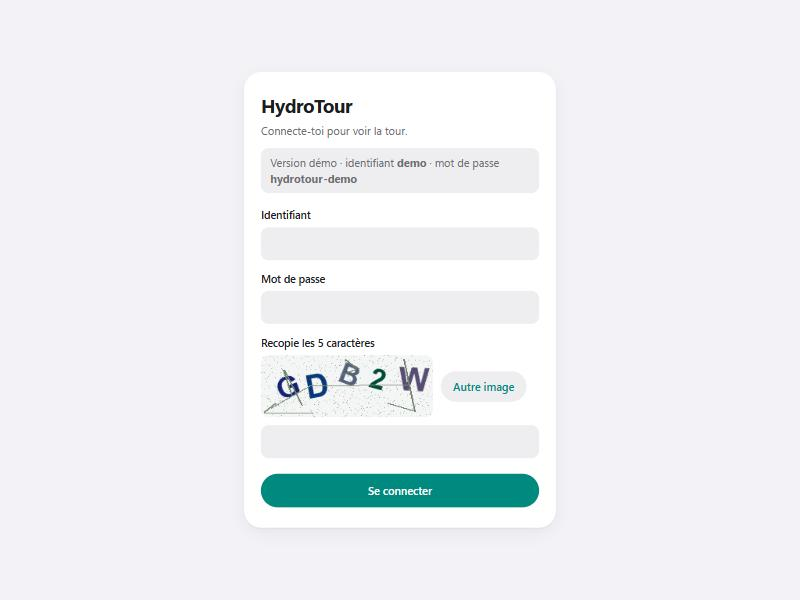
\includegraphics[width=0.75\textwidth]{img/inf/h_login.jpg}
\caption{Page de connexion de la démo, avec l'identifiant et le mot de passe rappelés et le captcha.}
\end{figure}

\subsubsection*{Le chemin d'une connexion}

Quand on ouvre la page, la garde regarde si la session est valide. Si elle ne l'est pas, elle renvoie vers la page de connexion. Le formulaire est accepté seulement si le captcha est juste, puis si le mot de passe correspond à l'empreinte. Je vérifie toujours le mot de passe, même quand l'identifiant est faux : le temps de réponse ne révèle donc pas si l'identifiant existe.

L'organigramme suivant décrit la connexion à la démonstration.

\begin{figure}[H]
\centering
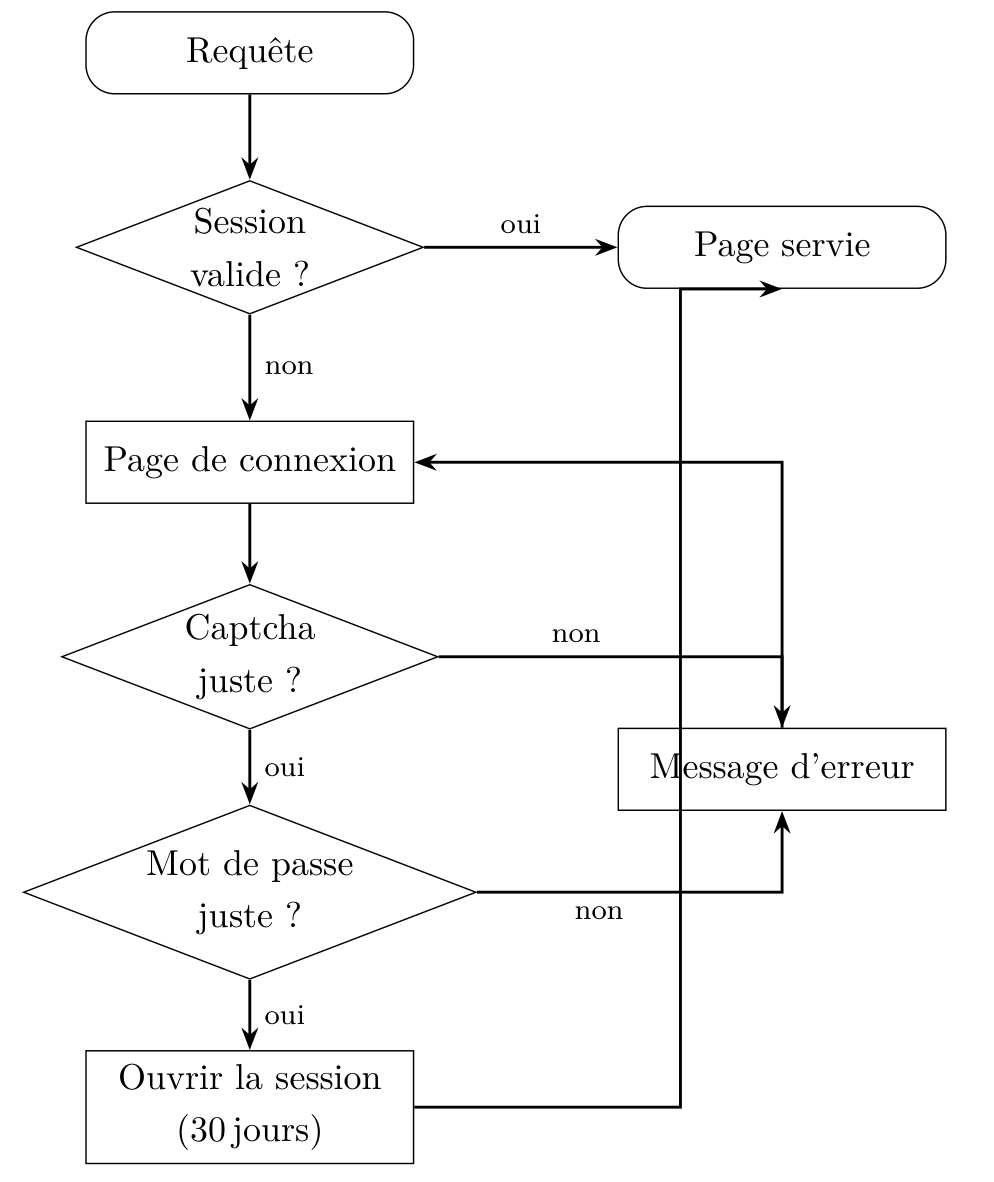
\includegraphics[width=0.6\textwidth]{img/inf/h_connexion.png}
\caption{Connexion à la démo (organigramme, ISO 5807).}
\end{figure}

\subsubsection*{Les routes du serveur}

Toutes les routes passent par la garde, sauf la page de connexion et l'image du captcha.

\begin{table}[H]
\centering
\small
\begin{tabularx}{\textwidth}{|l|l|Y|}
\hline
\textbf{Route} & \textbf{Méthode} & \textbf{Rôle} \\
\hline
\texttt{/} & GET & La page du dashboard \\
\hline
\texttt{/connexion} & GET, POST & Connexion (publique) \\
\hline
\texttt{/captcha.png} & GET & Image du captcha (publique) \\
\hline
\texttt{/api/latest} & GET & Dernière mesure, pompes, alertes, journal \\
\hline
\texttt{/api/history} & GET & Historique pour les courbes \\
\hline
\texttt{/api/pompe} & POST & Pompe principale ou dose à la main \\
\hline
\texttt{/api/pilotage} & GET, POST & Cycle, seuils de batterie, mode auto \\
\hline
\texttt{/api/culture} & GET, POST & Légume cultivé et date de plantation \\
\hline
\texttt{/api/stock} & GET, POST & Litres d'engrais A et B \\
\hline
\texttt{/api/batterie} & GET, POST & Capacité et tension de la batterie \\
\hline
\texttt{/api/etalonner} & POST & Étalonnage du pH et du niveau \\
\hline
\texttt{/api/acces} & GET, POST & Changer identifiant et mot de passe \\
\hline
\end{tabularx}
\caption{Routes de l'API.}
\end{table}

\subsubsection*{Le premier lancement}

Au premier lancement, la base est vide. Le serveur la remplit pour que la page ne soit pas vide à l'ouverture. Je génère trois jours d'historique, soit une mesure toutes les \qty{5}{min}, avec le script \texttt{fausses\_mesures.py} qui existait déjà. Je plante une tomate il y a \qty{30}{jours}, ce qui place la culture au stade floraison, avec les cibles de pH et d'EC correspondantes. Je mets enfin \qty{2}{L} dans chaque bidon d'engrais.

\naturecalc{simulation (valeurs du faux Arduino de la démonstration ; aucune mesure réelle)}
\begin{demonstration}[nombre de points d'historique]
\resultat{N = 864}
Le nombre $N$ de mesures (sans unité) vaut la durée $D$ (en h) divisée par le pas $p$ (en h) :
\[
N = \frac{D}{p}
\]
Avec $D = \qty{72}{h}$ et $p = \qty{5}{min} = \tfrac{1}{12}\,\unit{h}$ :
\begin{align*}
N &= \frac{\qty{72}{h}}{\frac{1}{12}\,\unit{h}}\\
N &= 72\times 12\\
N &= 864
\end{align*}
Le serveur en relève \num{870} dans l'historique, car quelques mesures en direct se sont ajoutées après le démarrage.
\end{demonstration}

Cette préparation ne se fait qu'une fois : si la base contient déjà des mesures, le serveur n'y touche pas.

% ---------------------------------------------------------------------
\Needspace{8\baselineskip}\subsection{Tests et résultats}

Cette sous-partie présente d'abord les vérifications que je fais, ensuite les données produites par la démonstration en tableaux et en courbes, puis ce que je constate et les limites. Elle se termine par le mode d'emploi pour lancer la démonstration.

\subsubsection*{Les vérifications}

Je teste d'abord que la connexion est bien exigée, puis que chaque route répond une fois la session ouverte. Pour ouvrir la session sans passer par le formulaire, j'utilise le client de test de Flask, qui écrit directement la session côté serveur. Je ne résous pas le captcha moi-même : c'est une protection anti-robot, et le formulaire de connexion reste à essayer à la main.

Le tableau suivant donne les résultats des essais.

\begin{table}[H]
\centering
\small
\begin{tabularx}{\textwidth}{|l|Y|l|}
\hline
\textbf{Essai} & \textbf{Attendu} & \textbf{Obtenu} \\
\hline
\texttt{/api/latest} sans session & refusé (401) & 401 \\
\hline
\texttt{/} sans session & redirigé vers \texttt{/connexion} & 302 \\
\hline
\texttt{/api/latest} avec session & données (200) & 200 \\
\hline
\texttt{/api/history} 72 h & environ 870 points & 870 \\
\hline
\texttt{/api/culture} & tomate, floraison & oui \\
\hline
\texttt{/api/stock} & 2 L et 2 L & oui \\
\hline
\texttt{/api/pilotage} & réglages (200) & 200 \\
\hline
\texttt{/} avec session & page complète & \qty{130782}{octets} \\
\hline
Bon mot de passe & accepté & oui \\
\hline
Mauvais mot de passe & refusé & oui \\
\hline
\end{tabularx}
\caption{Résultats des essais.}
\end{table}

\subsubsection*{La dernière mesure}

Voici la mesure renvoyée par \texttt{/api/latest} au moment des essais, avec l'état des pompes. La pompe principale tourne, car le cycle de \qty{15}{min} la met en marche, et les doseuses attendent que l'eau soit mélangée.

\begin{table}[H]
\centering
\small
\begin{tabularx}{0.7\textwidth}{|l|r|l|}
\hline
\textbf{Grandeur} & \textbf{Valeur} & \textbf{Unité} \\
\hline
pH & 5,91 & -- \\
\hline
EC & 1155 & \unit{\micro S/cm} \\
\hline
Température de l'eau & 20,5 & \unit{\celsius} \\
\hline
Température de l'air & 26,2 & \unit{\celsius} \\
\hline
Humidité & 75 & \unit{\percent} \\
\hline
Pression & 1012,7 & \unit{hPa} \\
\hline
Niveau d'eau & 77,9 & \unit{\percent} \\
\hline
Lumière & 0 & \unit{\percent} \\
\hline
Batterie (tension) & 12,967 & \unit{V} \\
\hline
Batterie (courant) & $-1{,}812$ & \unit{A} \\
\hline
Batterie (puissance) & $-23{,}5$ & \unit{W} \\
\hline
Batterie (charge) & 69,5 & \unit{\percent} \\
\hline
\end{tabularx}
\caption{Dernière mesure de la démo.}
\end{table}

\naturecalc{simulation (valeurs du faux Arduino de la démonstration ; aucune mesure réelle)}
\begin{demonstration}[courant de la batterie]
\resultat{I \approx \qty{-1,812}{A}}
La puissance $P$ (en W) vaut la tension $U$ (en V) fois le courant $I$ (en A) :
\[
P = U\times I
\]
J'isole $I$ :
\[
I = \frac{P}{U}
\]
\begin{align*}
I &= \frac{\qty{-23,5}{W}}{\qty{12,967}{V}}\\
I &\approx \qty{-1,812}{A}
\end{align*}
Cette valeur correspond à la mesure du tableau.
\end{demonstration}

\subsubsection*{Les statistiques sur 72 heures}

Je relève le minimum, le maximum et la moyenne de chaque grandeur sur l'historique de trois jours.

Le tableau suivant donne les statistiques de l'historique.

\begin{table}[H]
\centering
\small
\begin{tabularx}{\textwidth}{|l|r|r|r|l|}
\hline
\textbf{Grandeur} & \textbf{Minimum} & \textbf{Maximum} & \textbf{Moyenne} & \textbf{Unité} \\
\hline
pH & 5,82 & 6,02 & 5,92 & -- \\
\hline
EC & 1012 & 1184 & 1101 & \unit{\micro S/cm} \\
\hline
Eau & 20,3 & 22,1 & 20,97 & \unit{\celsius} \\
\hline
Air & 21,7 & 30,5 & 25,99 & \unit{\celsius} \\
\hline
Humidité & 66 & 93 & 79,99 & \unit{\percent} \\
\hline
Lumière & 0 & 99 & 22,5 & \unit{\percent} \\
\hline
Niveau & 65 & 83 & 74,9 & \unit{\percent} \\
\hline
Pression & 1011,4 & 1014,6 & 1013,0 & \unit{hPa} \\
\hline
Tension batterie & 12,61 & 13,84 & 13,01 & \unit{V} \\
\hline
Courant batterie & $-1{,}86$ & 2,83 & $-0{,}43$ & \unit{A} \\
\hline
Puissance batterie & $-23{,}5$ & 38,88 & $-5{,}28$ & \unit{W} \\
\hline
Charge batterie & 0 & 100 & 35,4 & \unit{\percent} \\
\hline
\end{tabularx}
\caption{Statistiques de l'historique (870 mesures).}
\end{table}

Le pH reste entre $5{,}82$ et $6{,}02$, donc dans la cible de la tomate à la floraison ($5{,}8$ à $6{,}3$). L'EC, elle, reste entre \qty{1012}{\micro S/cm} et \qty{1184}{\micro S/cm}, sous la cible de \qty{2000}{\micro S/cm} à \qty{2400}{\micro S/cm} : le pilote voudra donc doser de l'engrais en direct, ce qui rend la démonstration vivante.

\subsubsection*{Les courbes}

Je trace quatre grandeurs sur les \qty{72}{h} d'historique, une mesure toutes les \qty{30}{min}. Les données viennent directement de la route \texttt{/api/history}.

\begin{figure}[H]
\centering
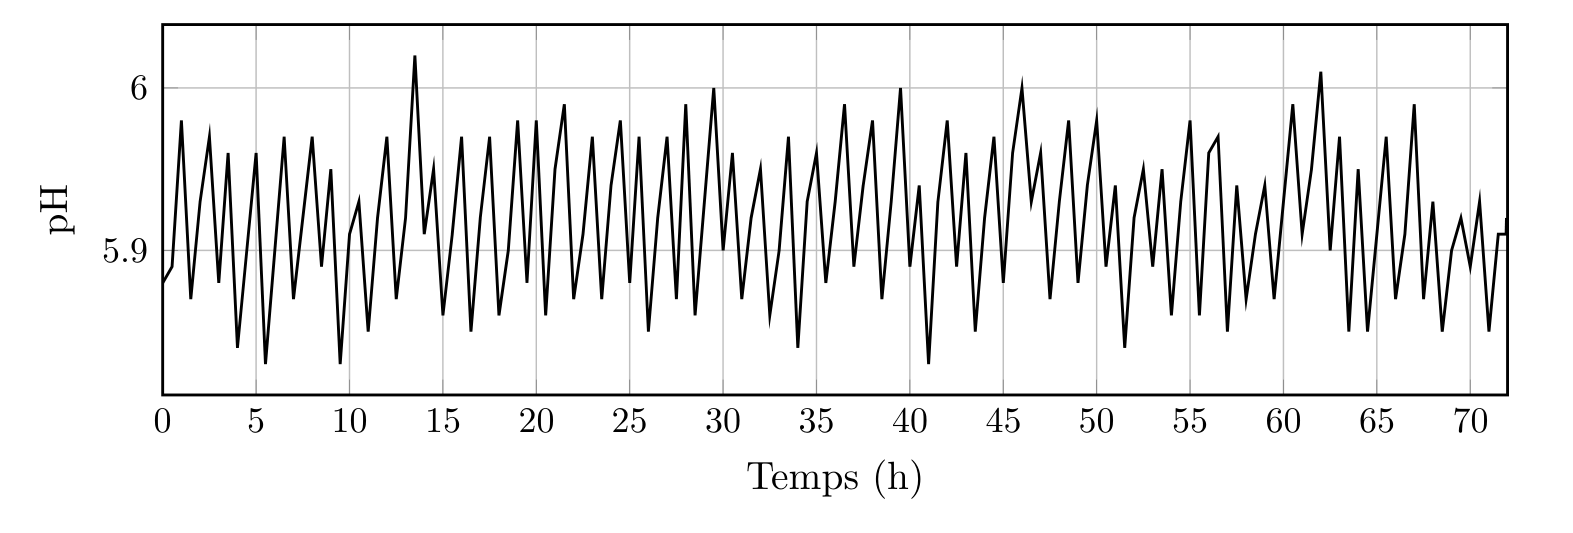
\includegraphics[width=0.9\textwidth]{img/inf/h_c_ph.png}
\caption{pH de la solution sur 72 h.}
\end{figure}

\begin{figure}[H]
\centering
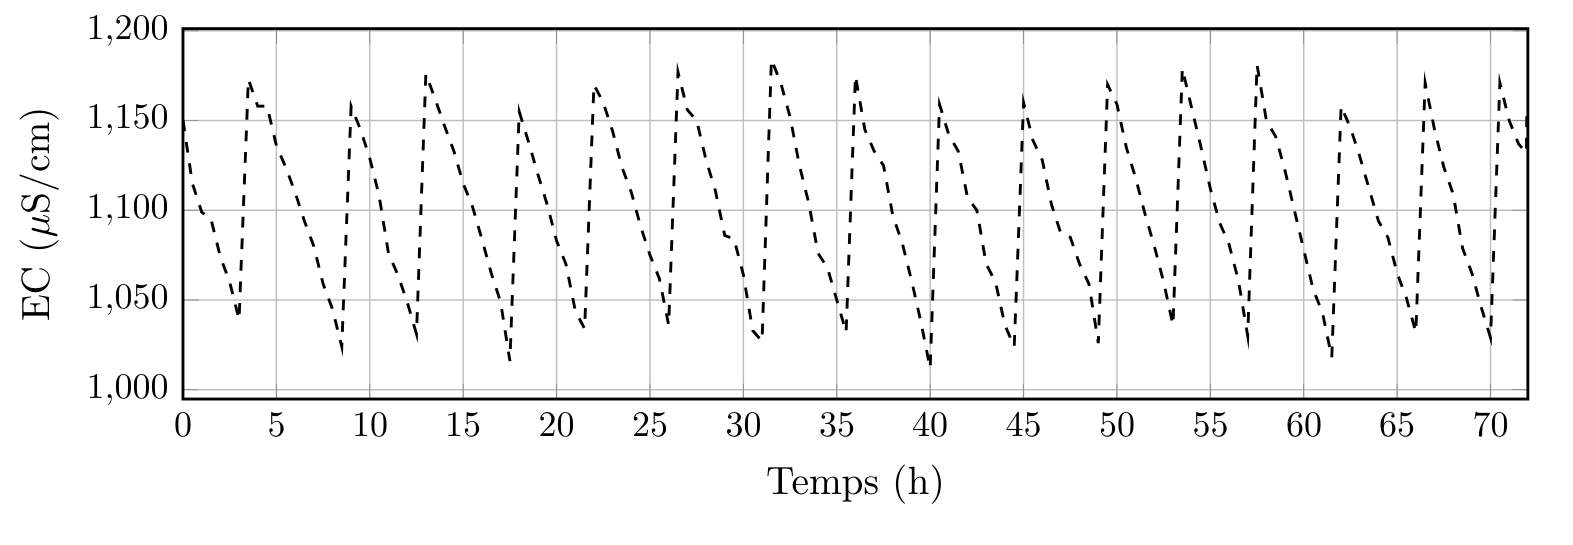
\includegraphics[width=0.9\textwidth]{img/inf/h_c_ec.png}
\caption{Conductivité de la solution sur 72 h.}
\end{figure}

\begin{figure}[H]
\centering
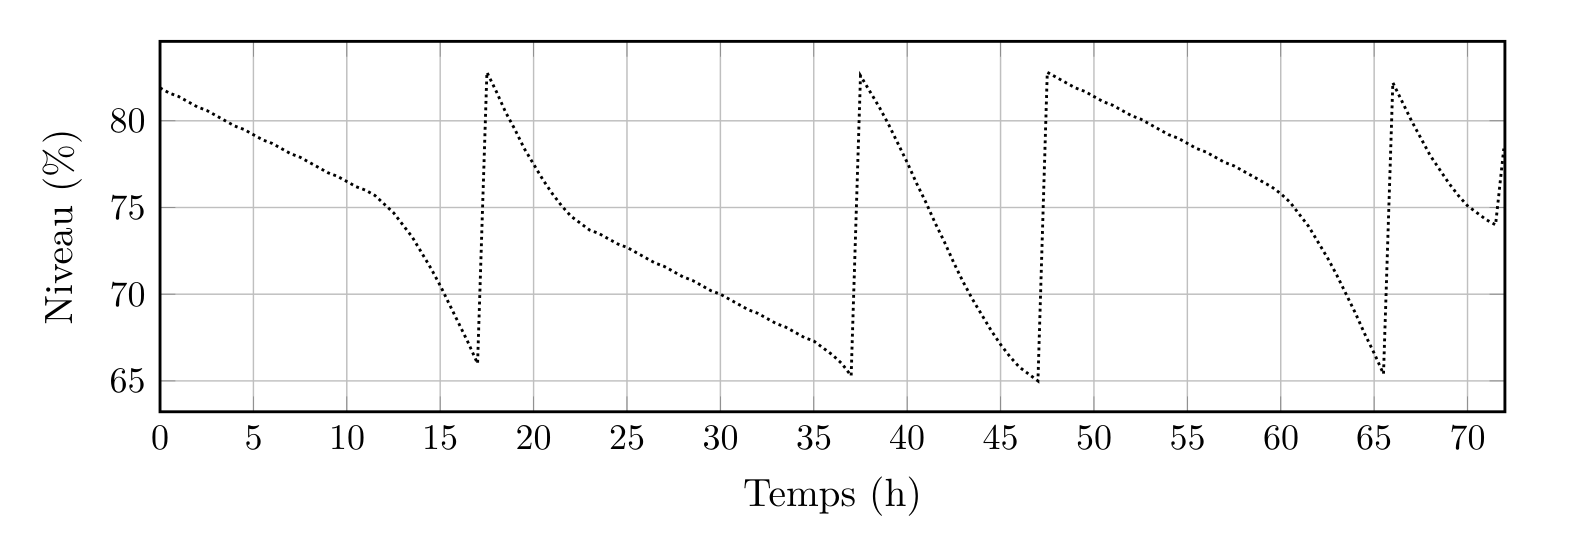
\includegraphics[width=0.9\textwidth]{img/inf/h_c_niv.png}
\caption{Niveau d'eau du réservoir sur 72 h.}
\end{figure}

\begin{figure}[H]
\centering
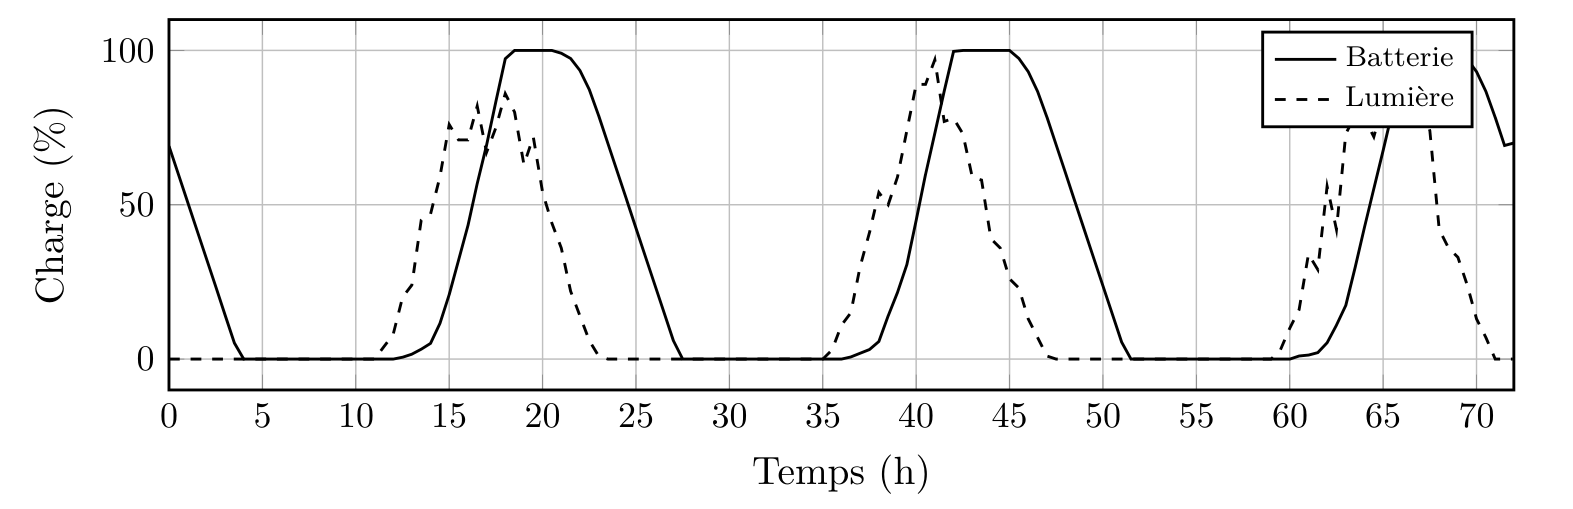
\includegraphics[width=0.9\textwidth]{img/inf/h_c_bat.png}
\caption{Charge de la batterie et lumière sur 72 h.}
\end{figure}

\subsubsection*{Ce que je constate et les limites}

Je constate d'abord que les courbes ont l'allure attendue : la lumière dessine un jour et une nuit, la batterie se charge le jour et se vide la nuit, le pH remonte puis redescend après chaque dose, et le niveau s'abaisse plus vite au soleil.

Deux limites sont à connaître. La première concerne l'historique : le script \texttt{fausses\_mesures.py} le génère sans pilote, avec une pompe qui tourne un quart d'heure sur deux, sans coupure de batterie. La charge descend donc jusqu'à \qty{0}{\percent} dans le passé, alors que le pilote en direct coupe la pompe à \qty{30}{\percent}. Il y a un saut entre la fin de l'historique et la première mesure en direct. La seconde limite concerne la connexion : je n'ai pas essayé moi-même le formulaire complet avec le captcha, car recopier un captcha est une action réservée à une personne. Les captures du dashboard de la sous-partie suivante viennent donc d'une copie statique de la page, qui embarque les données réelles du serveur de démo.

\begin{attention}
La démo tourne en temps réel : pour voir le pilote couper la pompe sous \qty{30}{\percent} ou doser de l'engrais, il faut la laisser tourner plusieurs heures, ou régler les seuils dans Paramètres.
\end{attention}

\subsubsection*{Lancer la démonstration}

Sur un ordinateur avec Python, j'ouvre le dossier \texttt{HYDROCODE/DEMO} et je lance \texttt{lancer\_demo.bat}. Ce fichier installe Flask et Pillow, puis démarre le serveur. J'ouvre ensuite \texttt{http://localhost:5000} et je me connecte avec \texttt{demo} et \texttt{hydrotour-demo}. Pour la rendre visible depuis Internet, il suffirait de publier le port 5001 avec Tailscale\ix{20} Funnel\ix{20}, comme pour la vraie tour : je ne l'ai pas fait.

\begin{aretenir}
La démo reprend le vrai serveur, le vrai pilote, la vraie page et la vraie sécurité. Elle fonctionne sans matériel, avec un compte fixe, et réagit comme la tour quand les pompes s'allument.
\end{aretenir}

% ---------------------------------------------------------------------
\Needspace{8\baselineskip}\subsection{Dashboard en ligne et captures}

Cette sous-partie explique d'abord comment je fabrique une copie statique du dashboard qui embarque les données de la démo. Elle présente ensuite les captures de chaque vue en lisant les valeurs qu'elles affichent, puis décrit la version publiée en ligne, avec ce qu'elle fait et ce qu'elle ne fait pas.

\subsubsection*{Une copie statique qui garde les données réelles}

Je cherche à obtenir des captures et une version en ligne sans dépendre du captcha ni d'un serveur qui tourne. La page \texttt{hydrotour.html} lit ses données avec la fonction \texttt{fetch} sur les routes \texttt{/api/...}. Je ne change donc rien à la page : j'ajoute avant elle un petit script qui remplace \texttt{fetch}. Ce script répond aux mêmes routes avec des données que j'ai relevées une fois sur le serveur de démo (client de test de Flask, session ouverte côté serveur). La page croit parler au serveur et passe en mode « En direct », comme sur la tour.

Le tableau suivant liste les routes imitées par la copie statique.

\begin{table}[H]
\centering
\small
\begin{tabularx}{\textwidth}{|l|Y|}
\hline
\textbf{Route imitée} & \textbf{Réponse du script} \\
\hline
\texttt{/api/latest} & dernière mesure, pompes, alertes, journal \\
\hline
\texttt{/api/history} & 942 mesures, filtrées sur la durée demandée \\
\hline
\texttt{/api/pilotage} & cycle 15/15 min, coupure \qty{30}{\percent}, reprise \qty{35}{\percent} \\
\hline
\texttt{/api/culture} & tomate plantée le 12 octobre \\
\hline
\texttt{/api/stock} & \qty{2}{L} d'engrais A et \qty{2}{L} d'engrais B \\
\hline
\texttt{/api/batterie} & \qty{6}{Ah}, \qty{12,8}{V} \\
\hline
\texttt{/api/pompe} (POST) & change l'état de la pompe en mémoire \\
\hline
\texttt{/api/acces}, \texttt{/api/etalonner} & refusés : pas de serveur derrière \\
\hline
\end{tabularx}
\caption{Routes imitées par la copie statique.}
\end{table}

Les mesures ont été prises à un moment précis, mais la page affiche « dernières 24 h » par rapport à l'instant présent. Je décale donc toutes les dates à chaque ouverture, pour que la dernière mesure tombe sur l'instant où la page s'ouvre.

\naturecalc{simulation (valeurs du faux Arduino de la démonstration ; aucune mesure réelle)}
\begin{demonstration}[décalage des dates]
\resultat{t'_i = t_i + \Delta\quad\text{avec}\quad \Delta = t_{\text{maintenant}} - t_{\text{dernière}}}
Je note $t_i$ la date de la mesure numéro $i$ dans les données relevées (en secondes depuis une origine fixe), $t_{\text{dernière}}$ la date de la dernière mesure et $t_{\text{maintenant}}$ l'instant d'ouverture de la page. Je veux que la dernière mesure tombe sur l'instant présent :
\[
t'_{\text{dernière}} = t_{\text{maintenant}}
\]
Je cherche un décalage $\Delta$ (en secondes) identique pour toutes les mesures, pour garder les écarts entre elles. Je pose :
\[
t'_i = t_i + \Delta
\]
Je l'écris pour la dernière mesure :
\begin{align*}
t'_{\text{dernière}} &= t_{\text{dernière}} + \Delta\\
t_{\text{maintenant}} &= t_{\text{dernière}} + \Delta\\
\Delta &= t_{\text{maintenant}} - t_{\text{dernière}}
\end{align*}
L'écart entre deux mesures est conservé :
\begin{align*}
t'_{i+1} - t'_i &= (t_{i+1} + \Delta) - (t_i + \Delta)\\
&= t_{i+1} - t_i
\end{align*}
Pour la vue 24 h, la page garde les mesures de date $t'_i \geq t_{\text{maintenant}} - \qty{24}{h}$. Avec une mesure toutes les \qty{5}{min} :
\begin{align*}
N &= \frac{\qty{24}{h}}{\frac{1}{12}\,\unit{h}}\\
N &= 24\times 12\\
N &= 288
\end{align*}
Les $942$ mesures relevées se décomposent en $864$ points d'historique et $942 - 864 = 78$ mesures en direct, soit $78\times\qty{10}{s} = \qty{780}{s} = \qty{13}{min}$ de fonctionnement du serveur avant le relevé.
\end{demonstration}

\subsubsection*{Les captures du dashboard}

Je prends moi-même les captures avec le navigateur intégré de l'application, dans une fenêtre de \qty{800}{px} de large. Chaque capture est lue en regard des données de la démo : les valeurs affichées sont celles du serveur, pas des valeurs écrites à la main.

La première vue est celle des mesures. Elle affiche en haut l'état de la liaison (« En direct »), puis une alarme quand une grandeur sort de sa cible. Ici l'alarme porte sur l'EC : \qty{1144}{\micro S/cm} contre une cible de \qty{2000}{\micro S/cm} à \qty{2400}{\micro S/cm}, ce qui correspond aux statistiques et explique pourquoi le pilote dose de l'engrais. Le pH, $5{,}94$, est dans sa cible de $5{,}8$ à $6{,}3$.

La figure suivante montre la vue Mesures, avec le bac et la solution nutritive.

\begin{figure}[H]
\centering
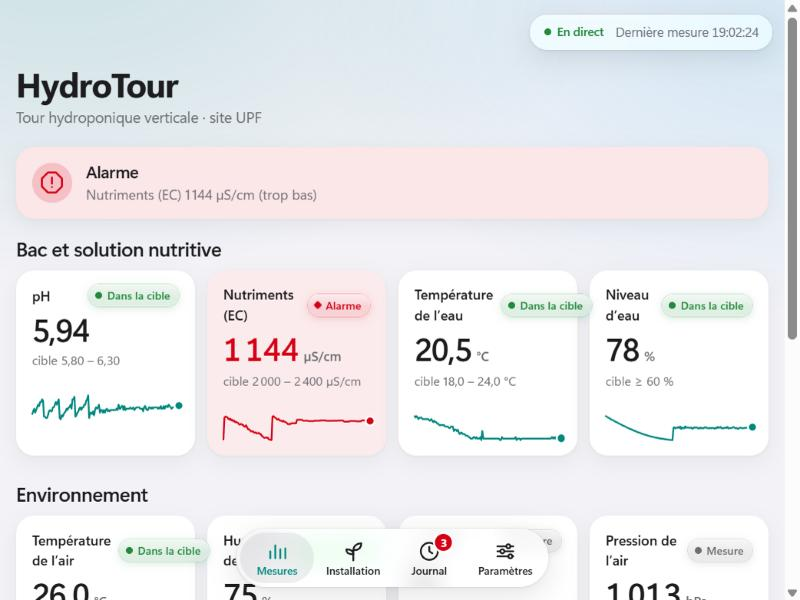
\includegraphics[width=0.8\textwidth]{img/inf/h_mesures.jpg}
\caption{Vue Mesures : bac et solution nutritive. L'EC est en alarme, le pH, la température de l'eau et le niveau sont dans leur cible.}
\end{figure}

Plus bas, la vue montre l'environnement (air, humidité, lumière, pression) et la batterie. Je contrôle l'autonomie affichée : la batterie contient \qty{49}{Wh} sur \qty{77}{Wh} et débite \qty{23,5}{W} (pompe et Raspberry).

\begin{figure}[H]
\centering
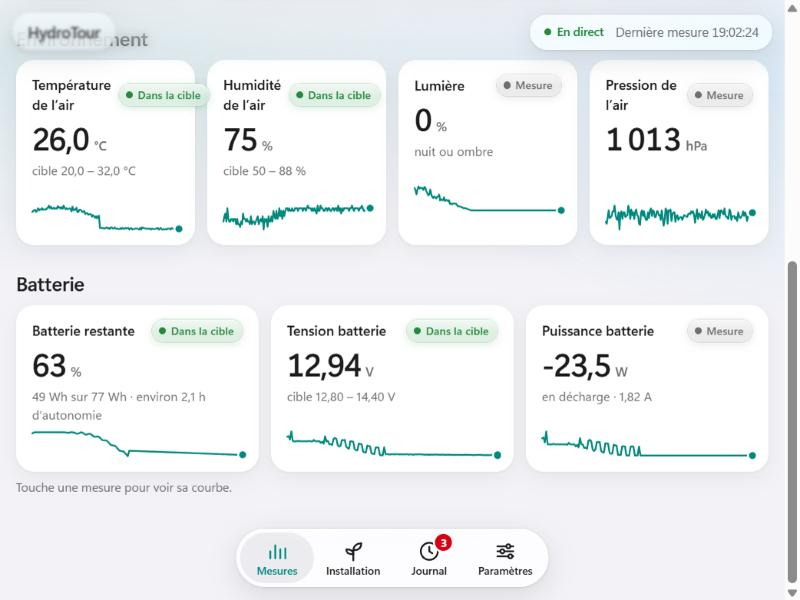
\includegraphics[width=0.8\textwidth]{img/inf/h_env.jpg}
\caption{Vue Mesures : environnement et batterie, avec l'autonomie estimée.}
\end{figure}

\naturecalc{simulation (valeurs du faux Arduino de la démonstration ; aucune mesure réelle)}
\begin{demonstration}[autonomie de la batterie]
\resultat{t \approx \qty{2,1}{h}}
L'autonomie $t$ (en h) vaut l'énergie restante $E$ (en Wh) divisée par la puissance de décharge $P$ (en W) :
\[
t = \frac{E}{P}
\]
L'énergie restante est la charge $\mathrm{SOC}$ (en \%) de l'énergie totale $E_0 = \qty{76,8}{Wh}$ :
\begin{align*}
E &= \frac{\mathrm{SOC}}{100}\times E_0\\
E &= 0{,}63\times\qty{76,8}{Wh}\\
E &\approx \qty{48,4}{Wh}
\end{align*}
La page arrondit la charge à partir d'une valeur un peu plus haute, ce qui donne \qty{49}{Wh}. Avec $P = \qty{23,5}{W}$ :
\begin{align*}
t &= \frac{\qty{49}{Wh}}{\qty{23,5}{W}}\\
t &\approx \qty{2,09}{h}
\end{align*}
La page affiche « environ 2,1 h ». Le courant affiché se contrôle de la même façon :
\[
\frac{\qty{23,5}{W}}{\qty{12,94}{V}} \approx \qty{1,82}{A}
\]
\end{demonstration}

La vue Installation montre la tour en trois dimensions, avec les plantes, le panneau solaire et le bac. Elle indique le stade de la culture (« Floraison, jour 30 »), qui vient de la date de plantation envoyée au serveur.

\begin{figure}[H]
\centering
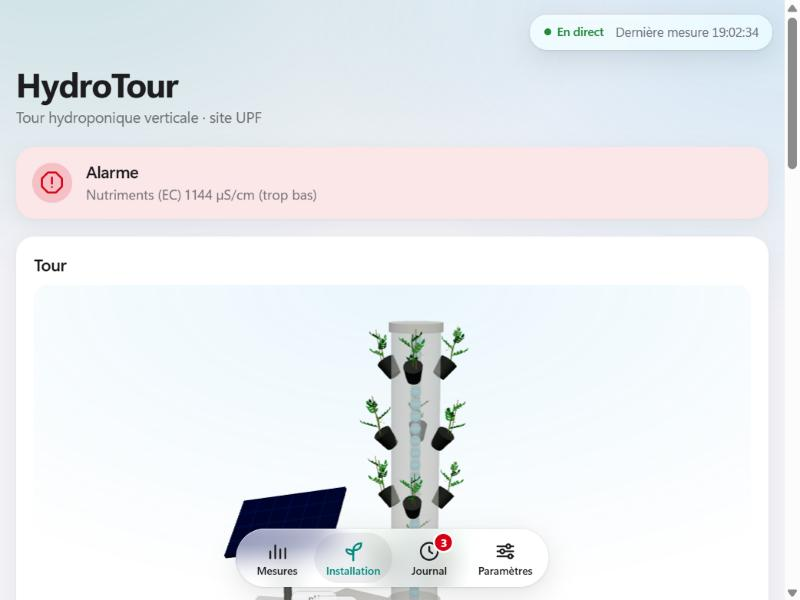
\includegraphics[width=0.8\textwidth]{img/inf/h_tour.jpg}
\caption{Vue Installation : la tour en 3D.}
\end{figure}

Sous la tour, le calendrier de la culture (tomate cerise, plantée le 12 octobre) colore chaque jour selon son stade. Je vérifie le numéro de jour : du 12 octobre au 11 novembre, il y a $19 + 11 = 30$ jours (les 19 jours restants d'octobre après le 12, puis 11 jours de novembre).

\begin{figure}[H]
\centering
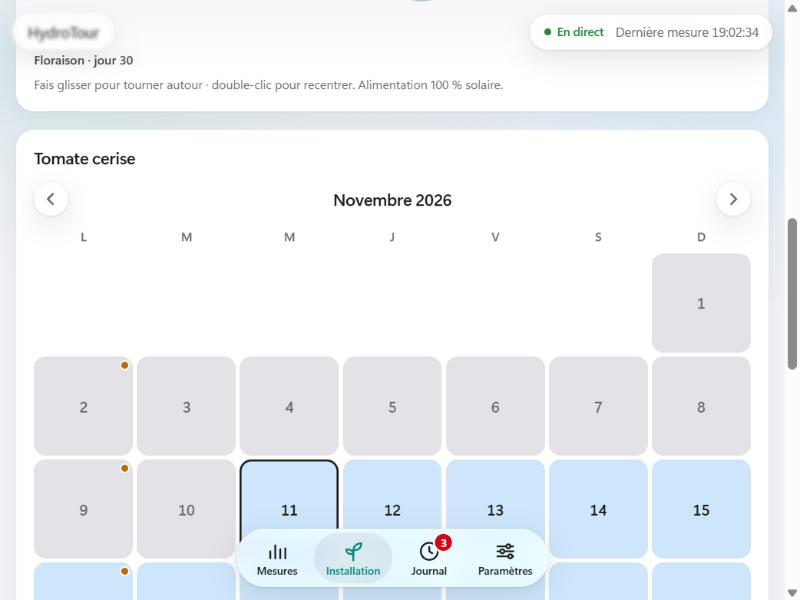
\includegraphics[width=0.8\textwidth]{img/inf/h_calendrier.jpg}
\caption{Vue Installation : calendrier de la culture.}
\end{figure}

La vue Journal liste les derniers événements du pilote (démarrage de la pompe, doses d'engrais et de pH-) puis un tableau des données récoltées par jour, sur 24 h, 7 j ou 30 j. Le tableau indique 942 mesures du 8 au 11 novembre.

\begin{figure}[H]
\centering
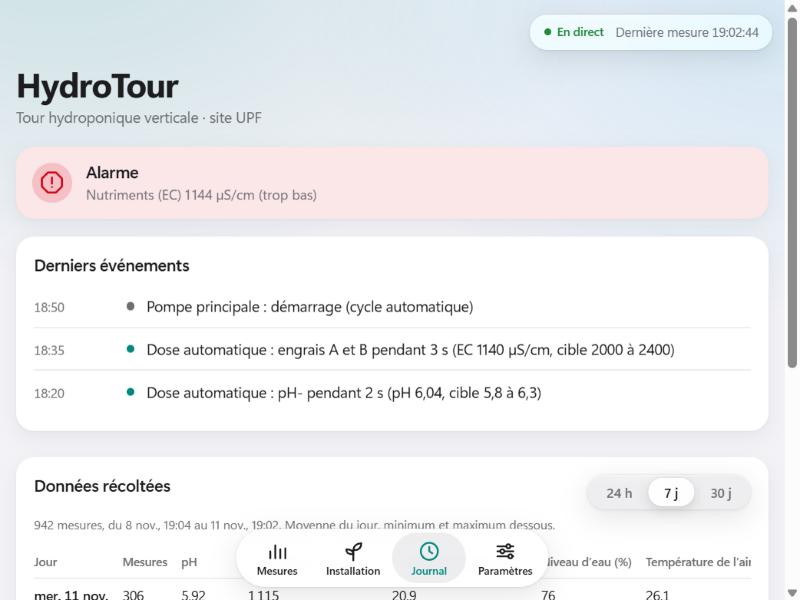
\includegraphics[width=0.8\textwidth]{img/inf/h_journal.jpg}
\caption{Vue Journal : événements du pilote et données récoltées.}
\end{figure}

\begin{attention}
Les trois lignes du journal de cette capture sont des exemples que j'ai écrits dans le style du pilote : le serveur utilisé pour le relevé n'avait pas encore produit d'événement. Les mesures et les cibles, elles, viennent de la démo.
\end{attention}

Enfin la vue Paramètres regroupe l'accès, le légume, la batterie, le pilotage et l'étalonnage. L'accès montre l'identifiant \texttt{demo}. Le pilotage affiche les valeurs par défaut du pilote : marche \qty{15}{min}, arrêt \qty{15}{min}, coupure de la batterie à \qty{30}{\percent} et reprise à \qty{35}{\percent}, soit le conseil du programme.

\begin{figure}[H]
\centering
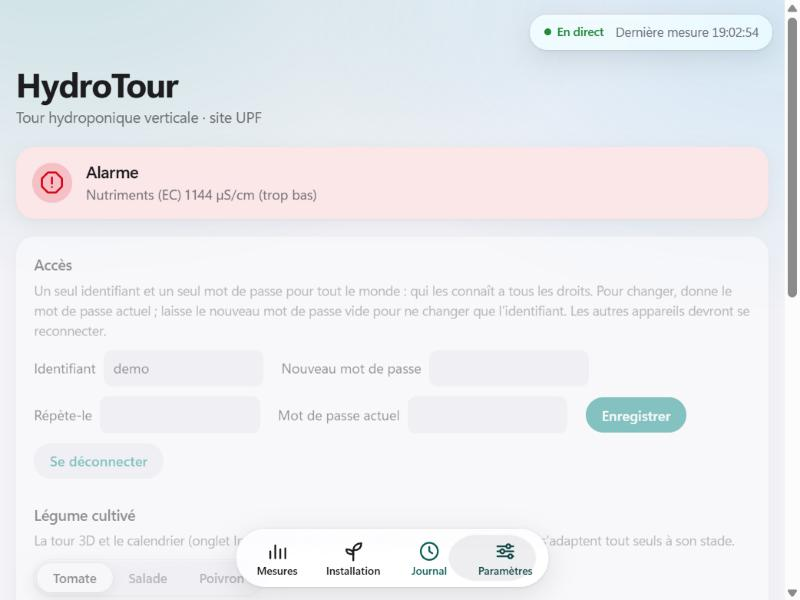
\includegraphics[width=0.8\textwidth]{img/inf/h_param.jpg}
\caption{Vue Paramètres : accès à la démo.}
\end{figure}

\begin{figure}[H]
\centering
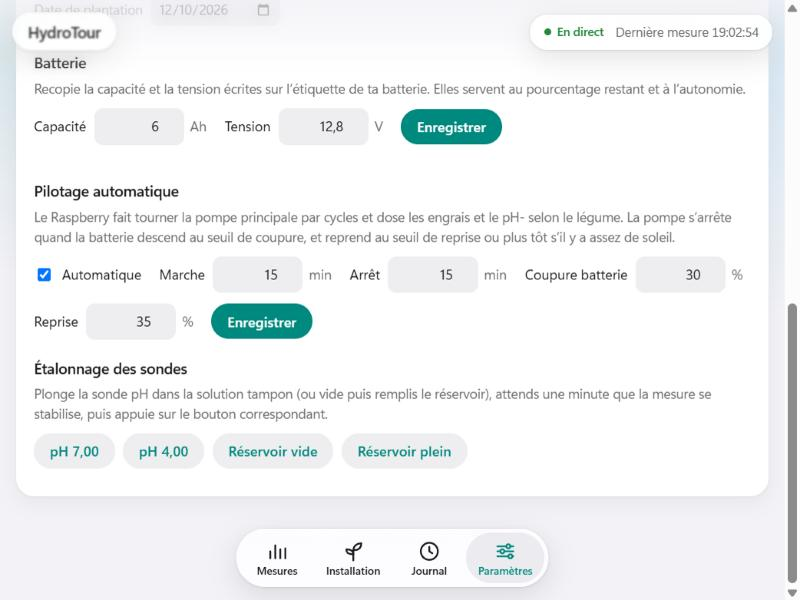
\includegraphics[width=0.8\textwidth]{img/inf/h_param2.jpg}
\caption{Vue Paramètres : batterie, pilotage automatique et étalonnage des sondes.}
\end{figure}

\subsubsection*{Le dashboard publié en artéfact}

Je publie le dashboard comme artéfact, une page web hébergée qui s'ouvre dans un navigateur sans rien installer. Depuis le 20 novembre 2026, la page publiée n'est plus une copie statique : c'est le fichier \texttt{hydrotour.html} de la tour, auquel j'ajoute une seule ligne qui pose un drapeau de démonstration. Le dashboard part alors dans son mode simulé, l'écran de pilotage et d'étalonnage reste affiché bien qu'aucun serveur ne réponde, et les actions qui demandent le matériel affichent un message au lieu de rester sans effet. La porte de connexion est ajoutée au même moment, par le programme \texttt{construire\_demo\_en\_ligne.py}. Il n'y a ainsi qu'une seule page à tenir à jour : \href{https://claude.ai/artifact/KExrrcoxh41KNf55szF4Wk}{\textbf{ouvrir le dashboard de démonstration}} (adresse complète : \url{https://claude.ai/artifact/KExrrcoxh41KNf55szF4Wk}). L'artéfact est privé : seules les personnes à qui je donne l'accès peuvent l'ouvrir.

Pour garder l'idée d'une copie avec identifiant et mot de passe, j'ajoute avant la page une porte de connexion : \texttt{demo} et \texttt{hydrotour-demo}. Il faut aussi recopier les cinq caractères du code affiché, dessiné dans la page avec des lettres penchées et des traits par-dessus (le bouton « Autre image » en génère un nouveau). Cette porte s'exécute dans le navigateur. Elle montre le même parcours que la vraie tour, mais elle ne protège rien, car le code de la page est lisible par celui qui l'ouvre. La vraie sécurité reste celle du serveur, décrite à la partie 8.6, et la page publiée ne contient aucune donnée réelle.

\begin{table}[H]
\centering
\small
\begin{tabularx}{\textwidth}{|l|Y|Y|}
\hline
 & \textbf{Serveur de démo} & \textbf{Artéfact} \\
\hline
Pilote et faux Arduino & oui, en temps réel & non \\
\hline
Données & générées en continu & figées, redatées à l'ouverture \\
\hline
Mot de passe & vérifié par le serveur & vérifié dans la page \\
\hline
Captcha & oui & oui, dans la page \\
\hline
Réglages et pompes & enregistrés dans la base & gardés dans la page seulement \\
\hline
Changer l'accès, étalonner & oui & refusé \\
\hline
Installation & Python, Flask, Pillow & aucune \\
\hline
\end{tabularx}
\caption{Comparaison des deux versions de la démo.}
\end{table}

Trois détails sont à connaître. Le bouton d'export du journal en fichier ne fait rien dans l'artéfact, car le lecteur d'artéfacts interdit les téléchargements lancés par une page. La vue 3D charge sa bibliothèque \texttt{three.js} depuis un réseau de diffusion, il faut donc une connexion Internet. Enfin, comme les données sont figées, la batterie et les courbes ne continuent pas d'évoluer : pour voir le pilote agir en temps réel, il faut lancer le serveur de démo.

\begin{aretenir}
La page du dashboard n'est pas modifiée : un script lui sert les données du serveur de démo, et une porte de connexion se place devant. Le serveur de démo prouve le fonctionnement, l'artéfact permet de le montrer partout.
\end{aretenir}

